\documentclass[11pt]{article}  
\usepackage[margin=1in]{geometry}
\usepackage{authblk}
\usepackage{hyperref}
\usepackage{graphicx}
\usepackage{amsmath}
\usepackage{amssymb}
\usepackage{framed,multicol}
\usepackage{algorithm2e}
\usepackage{soul}
\usepackage[usenames, dvipsnames]{color}

\usepackage{ltexpprt} 

\newcommand{\hlc}[2][yellow]{ {\sethlcolor{#1} \hl{#2}} }

\newcommand{\checkthis}[1]{{{\sethlcolor{Rhodamine}\hl{#1}}\xspace}}
\newcommand{\newtext}[1]{{\textul{#1}\xspace}}
\newcommand{\comment}[2][]{{\sethlcolor{green} \hl{#1}} {\color{JungleGreen} \it #2}\xspace}
\newcommand{\positiveinteger}{\ensuremath{\mathbb{Z}^+}\xspace}
\newcommand{\nonnegativeinteger}{\ensuremath{\mathbb{N}}\xspace}
\newcommand{\positivereal}{\ensuremath{\mathbb{R}^+}\xspace}
%\newcommand{\nonnegativereal}{\ensuremath{\mathbb{R}^+ \cup \{0\}}\xspace}
\newcommand{\nonnegativereal}{{\color{red} {\ensuremath{\mathbb{R}^+}}}}

\soulregister{\checkthis}{1}
\soulregister{\newtext}{1}
\soulregister{\comment}{2}


\title{Multi-Commodity Flow with In-Network Processing}
\author{Moses Charikar, Yonatan Naamad, Jennifer Rexford, and X. Kelvin Zou\\
Department of Computer Science, Princeton University\\
\texttt{\{moses,ynaamad,jrex,xuanz\}@cs.princeton.edu}}
\date{}

\begin{document}
\maketitle
\thispagestyle{empty}

\section{Introduction}
%%%
%%% Middleboxes are important
%%%
In addition to delivering data efficiently, today's computer networks often perform services on the traffic in flight to enhance security, privacy, or performance, or provide new features.  Network administrators frequently install so-called ``middleboxes'' such as firewalls, network address translators, server load balancers, Web caches, video transcoders, and devices that compress or encrypt the traffic.  In fact, many networks have as many middleboxes as they do underlying routers or switches.  Often a single conversation, or \emph{connection}, must traverse multiple middleboxes, and different connections may go through different sequences of middleboxes.  For example, while Web traffic may go through a firewall followed by a server load balancer, video traffic may simply go through a transcoder.  In some cases, the traffic volume is so high that an organization needs to run multiple instances of the same middlebox to keep up with the demand.  Deciding how many middleboxes to run, where to place them, and how to direct traffic through them is a major challenge facing network administrators.

%%%
%%% Dedicated appliances stink
%%%
Until recently, each middlebox was a dedicated appliance, consisting of both software and hardware.  Administrators tended to install these appliances at critical locations that naturally see most of the traffic, such as the gateway connecting a campus or company to the rest of the Internet.  A network could easily have a long chain of these appliances at one location, forcing all connections to traverse every appliance---whether they need all of the services or not.  In addition, placing middleboxes only at the gateway does not serve the organization's many \emph{internal} connections, unless the internal traffic is routed circuitously through the gateway.
%
%%%
%%% Network Function Virtualization
%%%
Over the last few years, middleboxes are increasingly \emph{virtualized}, with the software service separate from the physical hardware.  Middleboxes now run as virtual machines that can easily spin up (or down) on any physical server, as needed.  This has led to a growing interest in good algorithms that optimize the (i) \emph{placement} of middleboxes over a pool of server resources, (ii) \emph{steering} of traffic through a suitable sequence of middleboxes based on a high-level policy, and (iii) \emph{routing} of the traffic between the servers over efficient network paths~\cite{SIMPLE2013}.

%%%
%%% Combining the optimization problems
%%%
Rather than solving these three optimization problems separately, we introduce---and solve---a joint optimization problem.  Since server resources are fungible, we argue that each compute node could subdivide its resources arbitrarily across any of the middlebox functions, as needed.  That is, the \emph{placement} problem is more naturally a question of what fraction of each node's computational (or memory) resources to allocate to each middlebox function.  Similarly, each connection can have its middlebox processing performed on any node, or set of nodes, that have sufficient resources.  That is, the \emph{steering} problem is more naturally a question of how to decide which nodes should devote a share of its processing resources to a particular portion of the traffic.  Hence, the joint optimization problem ultimately devolves to a new kind of \emph{routing} problem, where we must compute paths through the network based on both the bandwidth and processing requirements of the traffic between each source-sink pair.  That is, a flow from source to sink must be allocated (i) a certain amount of bandwidth on every link in its path and (ii) a total amount of computation across all of the nodes in its path.

\subsection{The Problem}
We can abstract the flow in-network process problem in the following way: there is a flow demand with multi-sources and multi-sinks, and each flow requires a certain amount of in-network (MBox) processing. The in-network processing required for a flow is proportional to the flow size and without losing generality, we assume one unit of flow requires one unit of processing. For a flow from a source to a sink, we assume it is an aggregate flow so the routing and in-network processing for a flow are both divisible. In this model there are two types of constraints: edge capacity and vertex capacity, which represents bandwidth and MBox processing capacity. A feasible flow pattern satisfies: the sum of flows on each edge is bounded by the edge capacity, the sum of in-network process done at each vertex is bounded by the vertex capacity, and the processing done at all vertices for a flow should be equal to flow size and the processing has to be carried out by the flow.

Network design problems involve finding a network with a minimum cost that satisfies various properties, often related to routing and flow feasibility. The network design problem in this model is: for a multi-source and multi-sink flow demand, and a fixed amount of budget to install the processing capacities in the vertices, what is the optimal way to allocate them such that the flow pattern satisfies all the constraints.

Our model is a superset of multi-commodity flow model\cite{MCF}, that is, if we can solve this problem, we can naturally solve multi-commodity flow problem: simply assign each vertex with an infinite capacity it becomes an MCF problem. Many classic MCF design properties can be extended to this problem, such as MC-BB(multi-commodity buy-at-bulk) problem\cite{BuyAtBulk,Charikar05,Chekuri2007}. 
%This paper takes the second approach and show that the decision can be answered via generalized linear programming model for a fractional solution, and have a logarithm approximation for a more practical integer placement.

\begin{figure}[h]
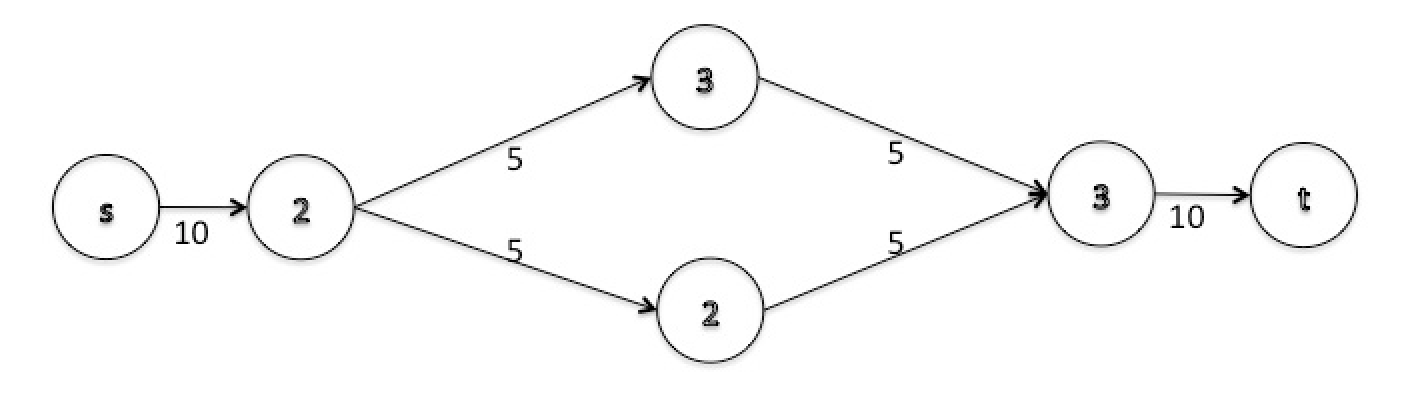
\includegraphics[width=\linewidth]{picture1.png} 
\caption{ \textbf{Example for the Graph Model: given the edge and vertex constraints, \textnormal{\{5,10\} }are edge capacities and \{2,3\} are vertex capacities, the maximum flow from source to sink in the example is 10, in this example all edges and vertices will be saturated.} }
 \end{figure}
\subsection{Notations}
To capture both the capacitated vertices and edges, we use the following notations:
a directed graph $G(V,E)$ where each edge $e\in E$ has an edge bandwidth $B(e)$, and each vertex $v\in V$ has a processing capacity $C(v)$. 

 


\subsection{The results in this paper}



\section{Flow Steering and Processing Allocation Problem}

%%%%%%%%%%%%%%%%%%%
%%%%%%%%%%%
%Basic problem
%%%%%%%%%%%
%%%%%%%%%%%%%%%%%%
\subsection{The basic problem}
We first solve the routing and steering problem for the above graph model: given all edge capacities $B(e)$ and vertex capacities $C(v)$ and a flow demand pattern $\mathbf{D}$, the optimization problem asks for a routing pattern with minimum congestion, the congestion can be interpreted in utilization. Like Max-flow model, we have capacitated edge constraints. However, our graph model has an extra constraint: vertex processing capacities, and it throttles the flow in a different manner: since a single flow is divisible and can be handled at different vertices, the flow is not constrained by a single node's processing power, but depending on all the nodes in the path(s). So a feasible flow pattern satisfies: (i) the edge capacities, (ii) the vertex capacities, and (iii) the relations between flow demand and processing demand. Without loss of generality, we assume the flow demand equals processing demand. 

Path-based formulation is built directly on the definition of the problem, and it takes paths as abstractions. We can also formulate an edge-based linear programming model. We can prove that they are equivalent(Proof see appendix). 

Notations: $f(U)$ is a convex function with a high penalty for high utilization. $B(e), C(v)$ are edge and vertex capacities, $D_i$ is the demand for flow i. For path-based formulation, $p(\pi,e)$ represents the processing work done at $v$ where $e\equiv(u,v)$, and $P_i$ is a set of path for flow i with $D_i$. For edge-based solution, $p_i(v)$ is the processing work done at v for flow $i$, and $w_i(e)$ is the process work demand at edge $e$ for flow $i$. 
Utilizations for edge and vertex are:
$U(e) = \frac{\sum\limits_i\sum \limits_{\pi\in P_i:e\in \pi} f(\pi)}{B(e)}=\frac{\sum\limits_{i} f_{i}(e)} {B(e)}$ and 
$U(v) = \frac{ \sum\limits_i \sum \limits_{\pi\in P_i} \sum \limits_{ e\in \pi} p(\pi, e) } {C(v)}=\frac{ \sum\limits_i p_i(v)}{C(v)}$.

\begin{minipage}[t]{0.45\textwidth}
\textit{Path-based formulation:}
  \begin{subequations}
\begin{align}
\text{Minimize:} & \sum \limits_{e} f(U(e)) + \sum \limits_{v} f(U(v)) \\  \nonumber
\text{Subject } &\text{to:} \\
\forall i,& \forall \pi\in P_i; \sum \limits_{e\in \pi} p(\pi, e) = f(\pi)\\
\forall i;& \sum\limits_{\pi\in P_i}f(\pi) = D_i\\
\forall \pi,&\forall e;p(\pi,e) \geq 0
\end{align}
\end{subequations}
  \end{minipage}
\hspace{0cm}
\begin{minipage}[t]{0.50\textwidth}
\textit{Edge-based formulation:}
  \begin{subequations}
\begin{align}
\text{Minimize:}&\sum \limits_{e} f(U(e)) + \sum \limits_{v} f(U(v)) \\ \nonumber
\text{Subject } &\text{to:}\\
\forall v \not= s,t,\forall i;& \sum\limits_{in}  f_i(e)=  \sum\limits_{out} f_i(e)\\
\forall v,\forall  i; p_i(v)& = \sum\limits_{in} w_i(e) - \sum\limits_{out} w_i(e) \\
\forall  i, \forall (s-v); &\sum\limits_v f_i(e)= D_i\\
\forall  i,\forall (s-v);& w_i(e)= f_i(e)\\
\forall  i,\forall (v-t);& w_i(e)= 0\\
\forall e,\forall i;w_i(e),& f_i(e)-w_i(e), p_i(v) \geq 0
\end{align}
\end{subequations}
\end{minipage}

Understand edge-based formulation: 2.2b is the same flow conservation, and 2.2c, g $p_i(v)$ shows the flow demand should be decreasing, 2.2d, e, f ensures the flow demand and process demand relations. 

%%%%%%%%%%%%%%%%%%%
%%%%%%%%%%%
%Flow size change
%%%%%%%%%%%
%%%%%%%%%%%%%%%%%%
\emph{Flow Size Changes after Processing:} the basic model shows that in-network processing does not affect the traffic size. However the change of flow size after processing is a common case in networking, for example, encryption increases the flow size while compression and transcoding decrease the traffic size\cite{Mogul1997}. We can capture this aspect and integrate into the optimization formulation. In generalized minimum cost circulation problem \cite{Wayne1999}, there is a gaining factor. We apply the same idea, but one key difference in our model is that flow size change only applies the gaining factor to part of the flow to be processed at the vertex. 

The change can be easily captured in the formulation, if there is a size change, at each vertex, we have $\sum\limits_{in} w(e) - \sum\limits_{out}  w(e) = p(v)$ and $\sum\limits_{out} (f(e) - w(e))-\sum\limits_{in}  (f(e) - w(e))= p(v)*r$, assume $r$ is a positive gaining factor. If $r=1$, we have exactly the flow conservation $\sum\limits_{out} f(e) -\sum\limits_{in}  f(e)= 0$. 

%%%%%%%%%%%%%%%%%%%
%%%%%%%%%%%
%Mutiple tasks as a DAG
%%%%%%%%%%%
%%%%%%%%%%%%%%%%%%

\subsection{Multiple tasks as a DAG}
In practice, a flow usually needs several different processes before sink. In the above formulation we assume there is only one task, or each vertex can run all types of flow processing where we can bundle all tasks into one task. Nevertheless if we have specialized hardware or two types of processing are preferred to be separated at different vertices, we need to revisit our formulation. 
We consider two common types of task relationships: serial and parallel. Serial tasks must be handled in a certain order while parallel tasks can happen in any order. We can satisfy the new requirement by modifying the optimization formulation. We consider two corner cases where there are N serial or N parallel tasks, and then we extend this to a general case where N tasks have a DAG relation. 

For $N$ serial tasks, we have $C^n(v); n\in\{1\dots N\}$ for $N$ different processing capacities. In optimization formulation 2.2, we can think of two different types of flows, pre-processed and post-processed, and in this model we have $N+1$ types of flows: pre-$n$-post-$(n-1)$ processed where $ n\in\{1\dots N\}$ and  fully processed flows. We can extend formulation 2.2 by adding $N-1$ process demands, in particular for 2.2c we extend to N different types of processing, $p_i^n= \sum\limits_{in} w_i^n(e) - \sum\limits_{out} w_i^n(e)$. Besides the same capacity and flow relation constraints, we also need $w_i^n(e) \geq w_i^{n-1}(e)$ where it reflects the sequence. The complexity of this formulation increases in a linear relation to the number of tasks $N$.
\begin{figure}
 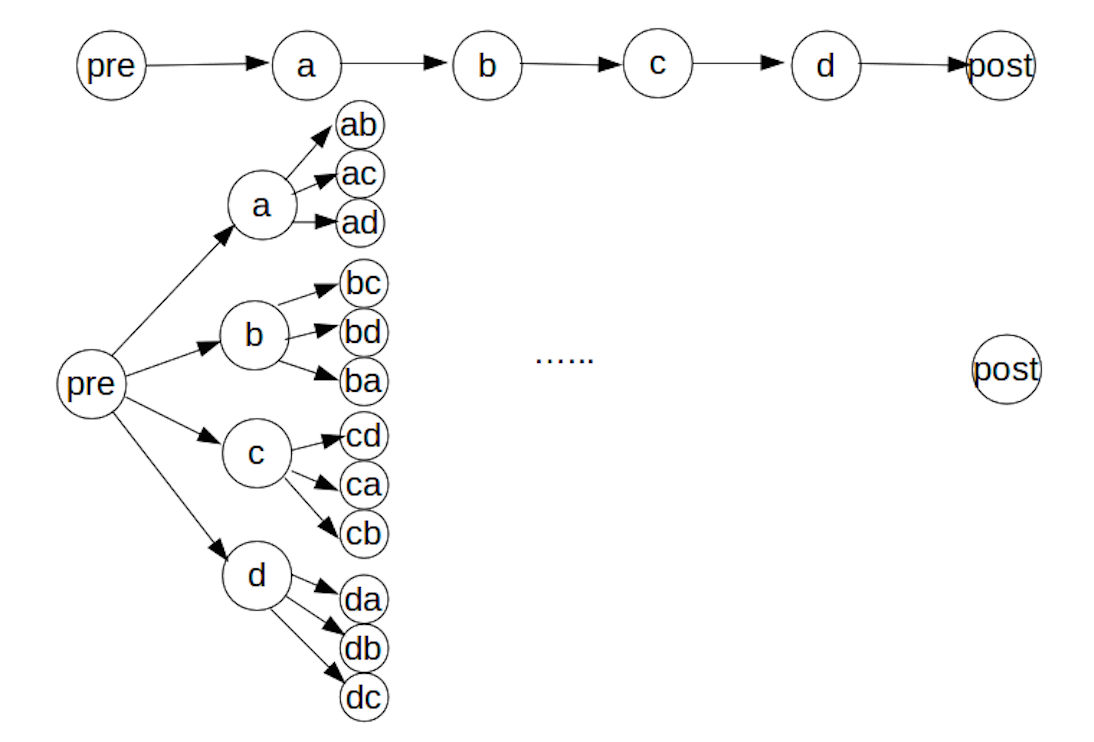
\includegraphics[width=\linewidth]{task.png}
 \caption{Up: serial tasks, Down: parallel tasks; a,b,c,d represents four different tasks and each link represents one dependency}
\end{figure}


For $N$ parallel tasks, again we have $C^n(v); n\in\{1\dots N\}$ for $N$ different processing capacities. Unlike serial relation, the number of types of flow grows exponentially, at most there can be $2^N$ types of flows. We have $O(2^N)$ inequalities represents the dependencies and $O(N)$ inequalities represents processing capacity relations.
% Surprisingly the complexity of the formulation also increases in a linear relation to the number of tasks N if we utilize the independence between tasks. The constraints are almost the same as above serial case except for that there is no sequential constraint like $w_i^n(e) \geq w_i^{n-1}(e)$. This optimization problem is similar to solve $N$ separate optimization problems and the $N$ problems are linked by the routing choice $f_i$ and the objective function. We argue that the optimization solution also provides with enough information for routing and processing decision; we can process the flow in the following manner: each flow has $N$ tags which indicates whether the part of the flow $n\in\{1\dots N\}$ is processed, and since the order can be arbitrary for $N$ processings, for each type of processing, it only needs to check its corresponding tag and make decisions independently. 

To generalize, if there are tasks with a DAG relation where each directed link $(p,q)$ represents a dependency of $q$ to $p$, there is an inequality relation $w_i^q(e) \geq w_i^p(e)$ for each link $(p,q)$. For any k parallel tasks, we need to build $O(2^k)$ branches and establish the relation using the method above.   


\section{Design Problem}
\input{Conclusion.tex}


\bibliographystyle{acm}
\bibliography{references}

\appendix
\section{Proof for equivalence between two LPs section2.1}
Proof sketch: we first show that we can compose an \emph{edge-based} solution based on a \emph{path-based} solution and vice versa for a single flow, and then show that we can iteratively place multi-commodity flows. 
\begin{enumerate}
\item show \emph{Direction A:} If there is a \emph{path-based} LP solution, there is an \emph{edge-based} solution.
\item show \emph{Direction B:} If there is an \emph{edge-based} LP solution, there is a \emph{path-based} solution using path decomposition.
\item show the formulations for multi-commodity flows are also equivalent via extending the above approach.
\end{enumerate}

\subsection{\emph{path-based} solution $\rightarrow$ \emph{edge-based} solution}
\begin{proof}
we show that we can easily convert path-based solution to edge-based solution and all the constraints in edge-based formulation hold.

For each edge e, $f(e) =\sum\limits_{\pi\in P: e\in \pi} f(\pi)$.

For each vertex v, $w(e) = \sum\limits_{\pi\in P: e'\in \pi, e' \leq e} p(\pi, e')$ ($e'\leq e$ means e' is topologically at or after e on the path $\pi$).(A.2c)

Flow conservation holds $ \sum\limits_{(u,v)\in E} f(e) $=$ \sum\limits_{\pi\in P, v\in \pi} f(\pi)$ = $\sum\limits_{(v,w )\in E} f(e)$.(A.2b)

Constraints in terms of $B(e), C(v)$ also hold. (A2d,2e)

Relations between $w(e), f(e)$ also hold: $w(e)= \sum\limits_{\pi\in P: e'\in \pi, e' \leq e} p(\pi, e')\leq \sum\limits_{\pi\in P: e\in \pi} f(\pi) = f(e) $, and $w(s,v)=f(s,v)$ and $w(v,t)=0$ are special cases.(A.2f,2g,2h)

\end{proof}

\subsection{\emph{edge-based} solution $\rightarrow$ \emph{path-based} solution}
To prove this; we need to show:
\begin{enumerate}
 \item We can always construct a path if there is some residual flow left in the graph.
 \item All constraints holds for the updated residual graph.
 
\end{enumerate}

Setup:
A directed graph $G(V,E)$ with an \emph{edge-based} LP solution, where $f(e)$ is the flow for each edge, $w(e)$ is workload demand at the same edge and $p(v)$ process work done at each vertex v. Build a new graph $G'$: all vertices $V$, and for $\forall e\in E $, if $f(e) >0$, we put a direct edge $e$ in the graph. To help proof, divide a flow into two states, processed and unprocessed $f^1$ and $f^2$; in terms of flow volume $f^1=w$ and $f^2=f-w$. 
\begin{lemma} loops for flows $f^1$ and $f^2$ respectively can be cancelled via flow cancellation without any side effect. 
\end{lemma} 

\begin{proof} it is similar to flow cancellation in a simple graph model: 

(i) for e=(u,v) whereas $min(f^1) >0$, we can simply cancel the unprocessed flow demand by small amount $\epsilon$, and it does not affect the outcome of the flow outside the loop, while we can reduce the flow load and workload demand in the loop without side effect. 

(ii) for e=(u,v) whereas $min(f^2)>0$, we can cancel the processed flow demand by small amount $\epsilon$, and this does not affect the outcome of the flow outside of the loop while we can reduce the flow load in the loop without side effect. 

The intuition behind this is that loop exists due to that some flow needs to borrow some processing capacity from some node(s), so it would ``detour" a flow in an unprocessed state and get back the flow in a processed state. 
\end{proof}

Introduce an intermediate variable $\rho$ for each edge e where $\rho_{e} = \frac{w(e)}{f(e)} = \frac{ f^1} {f^1+f^2 }$. Run flow loop cancellation for $f^1$ and $f^2$ respectively in $G'$.

\textbf{Note:} after loop cancellation we may still have loops for $f$ as a unitiy. 
\begin{lemma}
$\rho$ has the following property: if there is a cycle for unity flow $f$, there is always at least one edge with $\rho =1$ and one edge with $\rho =0$.
\end{lemma}
\begin{proof}
 This can be easily inferred from Lemma A.1.
\end{proof}



\begin{algorithm}[ht]
  \SetAlgoLined\DontPrintSemicolon
   \KwData{$G'(V, E)$, $ w(e)$, $f(e)$ for $\forall e \in E$ and $p(v)$ for $\forall v \in V$ }
\KwResult{$f(\pi)$, $p(\pi,v)$ where $v\in\pi$ }
\SetKwFunction{path}{Path Construction} \label{path construction}
  \SetKwFunction{flow}{Flow Placement} \label{flow placement}
  \SetKwProg{myalg}{Algorithm}{}{}
  \myalg{\path{}}  {
\emph{//Construct path from $s\rightarrow v$ and $v\rightarrow t$}\;
From v run backward traversal, pick an incoming directed edge with $ max( \rho_{in} )  $ where $\rho_{in} \equiv \frac{ w(e_{in})}{f(e_{in})}$\;
From v run forward traversal, pick an outgoing directed edge with $ min(\rho_{out} ) $ where $\rho_{out} \equiv \frac{ w(e_{out})}{f(e_{out})} $\;
 \KwRet $\pi$\;}{}
%   \nl \KwRet $\pi$\;}{}
  \setcounter{AlgoLine}{0}
  \SetKwProg{myproc}{Algorithm}{}{}
  \myproc{\flow{}}{
  \BlankLine
\While{$\exists v; p(v) >0$}
{
 \emph{//path representation $\pi\equiv <v_1, \dots, v_k> \equiv <e_1, \dots, e_{k-1}>$}\;
 $\pi$ = \path{}\;
$f(\pi) = \min\{f^1(e^a), f^2(e^b), p(v)\},\; e^a\in <e_1,\dots, u\rightarrow v>, e^b\in <v\rightarrow w,\dots,e_{k-1}>$\;
	$p(\pi, v)=f(\pi)$\;
 	\For{$u\in \pi$ and $u\not=v$ }
	{
	$p(\pi, u)=0$\;
	}
	$C(v) = C(v) - f(\pi)$\;
	$p(v) = p(v) - f(\pi)$\;
	\For{$i \leftarrow 1 $ \KwTo $k-1$}{
	$f(e_i)=f(e_i)-f(\pi)$\;
	$B(e_i)=B(e_i)-f(\pi)$\;
	}
}
}
\caption{Path Decomposition}
\end{algorithm}


\begin{lemma}  [Path Construction] Algorithm \ref{path construction} can always generate path with non-zero flow from source to sink if there exists any $v$ where $p(v) >0$. \end{lemma}
\begin{proof}
\textit{First}, from Lemma A.2, the path cannot loop a cycle twice from [Path Construction]. Since downstream traversal keeps picking $\min \rho$ while upstreaming traversal keeps picking $\max \rho$, so we never pick the same edge twice. Since $p(v)>0$ so at the same node there must be one upstream edge with $\rho>0$ and downstream edge with $\rho<1$. Since the same edge is never picked twice so there is no loop in terms of $f^1$ and $f^2$. The path consists of two DAGs, one is from source to $v$ and one is from $v$ to sink, the path is a DAG as well.

\textit{Second} we need to show for a certain path $\pi; f(\pi)>0$. Since $ f(\pi) =  \min\{f^1(e^a), f^2(e^b), p(v)\}$; at node v where $p(v)>0$, so we have $f^1(e_{in})>0$ and $f^2(e_{out})>0$ at vertex $v$. Since we only pick $\max\{\rho\}$ for upstream traversal, so for $\forall e^a; f^1(e^a)>0$. The same reason we have $\forall e^b; f^2(e^b)>0$.

\end{proof}

\begin{lemma} [Flow Placement] Algorithm \ref{flow placement} conserves all the constraints for the reduced graph.
\end{lemma}
\begin{proof}
we show that all the constraints are satisfied:

for A.2b:
$\forall v \in \pi; \sum\limits_{in}  f(e) - \sum\limits_{out} f(e)=\sum\limits_{in \not=e_i}  f(e) - \sum\limits_{out\not=e_{i+1} } f(e) +[f(e_i)-f(\pi) ] - [f(e_{i+1}) -f(\pi)] = 0 $

A.2d:
$\forall e \in \pi; f(e) = f(e)-f(\pi) \leq B(e)-f(\pi)=B^{new}(e)$ 

A.2e:
$\forall v \in \pi; p(v) - f(\pi) \leq C(v) - f(\pi) =C^{new}(v)$

A.2f and A.2g are ensured by the algorithm, since $v\not=s $ and $ v\not=t$.

A.2h constraints are satisfied by numerical relations.
\end{proof}

\subsection{Multi-Commodity Flow}
For MCF, we can use the same approach above. For a graph with K source-sink paired flows,  we iterate $i = 1 \dots K$, for each flow we genrate a $G'$ and exhaustively decompose paths for $f_i$ and it is easy to see that all the constraints still hold after flow $i$ has been removed.  
In particular, we have :
A.2b, A.2c, A.2f and A.2g  hold for all the flows left after one flow is removed;
A.2d: $\forall i,\forall e;  \sum\limits_{l=i}^K f_l(e) - f_i\leq B(e) - f_i(e)$;
A.2e: $\forall i,\forall v;  \sum\limits_{l=i}^K p_l(v) -p_i(v)\leq C(v) - p_i(v)$.


\end{document}